\chapter{Process}
\section{目的}
掌握在一个进程中创建另一个进程的方法。
\section{目标}
编写一个程序,并在这个程序中创建一个新的进程,在父进程中每秒输出一个字符,同时子进程也每秒输出一个字符。
\section{实验过程}
\subsection{准备知识}
\subsubsection{创建子进程的方式}
在一个进程中创建一个子进程可以有三种方式:
\begin{enumerate}
\item
system

其执行过程如Figure \ref{pro-system}所示。
\item
exec

其执行过程如Figure \ref{pro-exec}所示。
\item
exec+fork

其执行过程如Figure \ref{pro-fork}所示。
\end{enumerate}
\begin{figure}
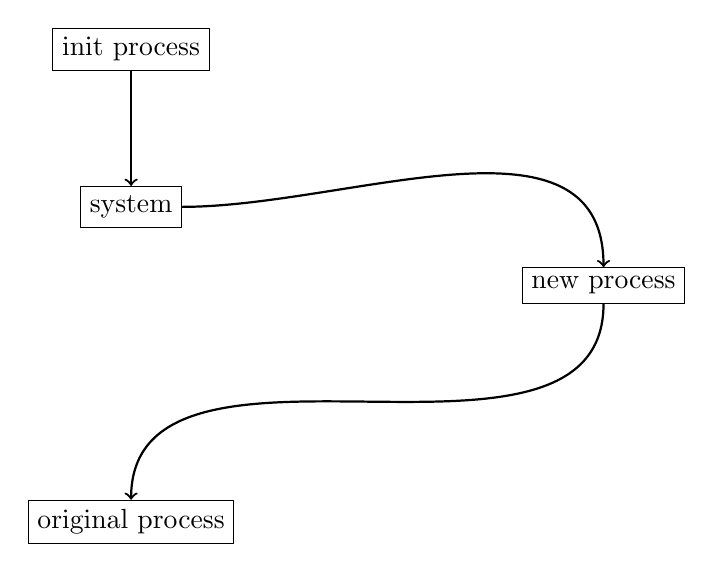
\begin{tikzpicture}
\node (i) [rectangle,draw] at (0,6) {init process};
\node (f) [rectangle,draw] at (0,4) {system};
\node (o) [rectangle,draw] at (0,0) {original process};
\node (n) [rectangle,draw] at (6,3) {new process};
\draw [->,thick] (i)--(f) ;

\draw [thick,->] (f) to[out=0,in=90]  (n);
\draw[thick,->] (n) to[out=270,in=90] (o);
\end{tikzpicture}
\caption{system图示}
\label{pro-system}
\end{figure}

\begin{figure}
\begin{tikzpicture}
\node (i) [rectangle,draw] at (0,6) {init process};
\node (f) [rectangle,draw] at (0,4) {exec};
\node (o) [rectangle,draw,dashed] at (0,0) {original process};
\node (n) [rectangle,draw] at (8,0) {new process};
\draw [->,thick] (i)--(f) ;

\draw [thick,->] (f) to[out=0,in=90]  (n);
\draw [dashed,thick,->] (f) to[out=270,in=90] node{X} (o);
\end{tikzpicture}
\caption{exec图示}
\label{pro-exec}
\end{figure}

\begin{figure}
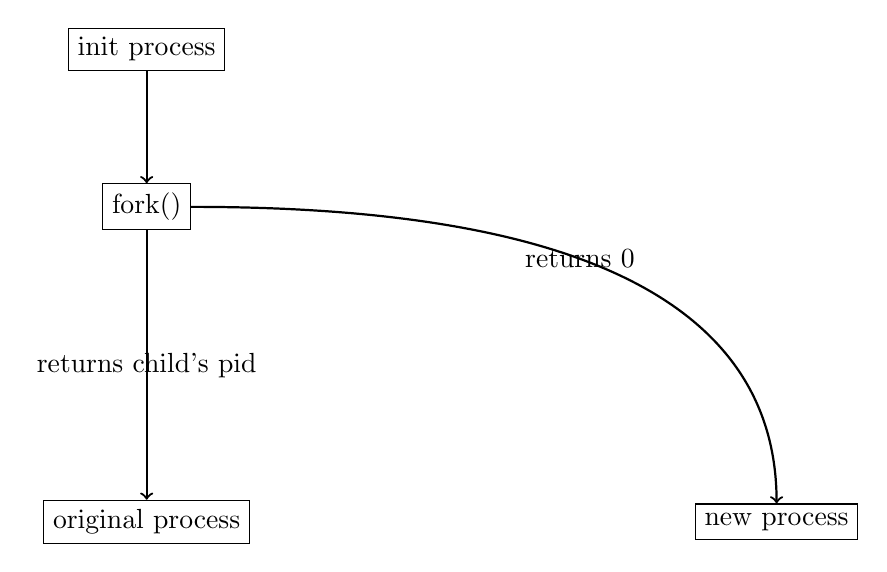
\begin{tikzpicture}
\node (i) [rectangle,draw] at (0,6) {init process};
\node (f) [rectangle,draw] at (0,4) {fork()};
\node (o) [rectangle,draw] at (0,0) {original process};
\node (n) [rectangle,draw] at (8,0) {new process};
\draw [->,thick] (i)--(f) ;

\draw [thick,->] (f) to[out=0,in=90] node{returns 0} (n);
\draw [thick,->] (f) to[out=270,in=90] node{returns child's pid} (o);
\end{tikzpicture}
\caption{fork图示}
\label{pro-fork}
\end{figure}
\subsection{使用fork的方式完成本实验}
请过man 3 fork来查看相关函数原型。
本实验的一个参考代码如Figure \ref{pro-ps}所示。
\begin{figure}
\begin{verbatim}
#include<unistd.h>
#include<stdlib.h>
#include<stdio.h>

void fmt(char st, char ed);
int main(){
	
	printf("I will fork a progress.\n");
	pid_t pid=fork();
	switch(pid){
		case -1:
			printf("error!");
			break;
		case 0:
			//printf("I am child.\n");
			fmt('a','z');
			break;
		default:
			//printf("I am parent.\n");
			fmt('A','Z');
			break;
			
	}
	if(pid!=0){
		int stat;
		pid_t child;
		child=wait(&stat);
		printf("\nthe child(pid=%d) has finished.\n",child);
		if(WIFEXITED(stat)!=0){
			printf("child exit with code:%d\n",WEXITSTATUS(stat));
		}else{
			printf("child terminated abnormally.\n");
		}
	}
	exit(0);
}

void fmt(char st, char ed){
	for(char a=st; a<=ed;a++){
		fputc(a,stdout);
		//
		sleep(1);
	}
}
\end{verbatim}
\caption{非严格意义的交替输出}
\label{pro-ps}
\end{figure}

\subsection{DEBUG}
\textcolor{red}{What!?}
Figure \ref{pro-ps}所示代码与我们期待的结果竟然不一样?这是为什么呢?请大家一起来查找问题的原因所在吧。